%% The Recursive Observability Filter
%% arXiv preprint -- first draft
%% Build:  latexmk -pdf main.tex     (or  make )

\documentclass[11pt]{article}

\usepackage[a4paper,margin=1in]{geometry}
\usepackage[T1]{fontenc}
\usepackage{lmodern}            % scalable outlines, not bitmaps, in the final PDF
\usepackage{amsmath,amssymb,amsthm}
\usepackage{graphicx}
\usepackage{booktabs}
\usepackage{array}
% Ragged-right paragraph column: narrow table cells justify badly.
\newcolumntype{L}[1]{>{\raggedright\arraybackslash}p{#1}}
\usepackage{xcolor}
\usepackage[font=small,labelfont=bf,skip=6pt]{caption}
\usepackage{tikz}
\usetikzlibrary{arrows.meta,positioning,calc}
\usepackage{microtype}          % tightens justification; kills most overfull lines
\usepackage[round,authoryear]{natbib}
\usepackage[colorlinks=true,allcolors=blue!60!black]{hyperref}

% ------------------------------------------------------- page discipline
% No single line of a paragraph left stranded at a page boundary, and no
% figure allowed to strand the text that introduces it.
\widowpenalty=10000
\clubpenalty=10000
\displaywidowpenalty=10000
\renewcommand{\topfraction}{0.85}
\renewcommand{\bottomfraction}{0.70}
\renewcommand{\textfraction}{0.12}
\renewcommand{\floatpagefraction}{0.72}
\setlength{\emergencystretch}{2em}

% ---------------------------------------------------------------- notation
\newcommand{\Icap}{I}                 % capability
\newcommand{\Reg}{R}                  % regulation
\newcommand{\Obs}{O}                  % observability
\newcommand{\Icrit}{I_{\mathrm{crit}}}
\newcommand{\Ofloor}{O_{\mathrm{floor}}}
\newcommand{\Odet}{O_{\mathrm{detectable}}}
\newcommand{\Arec}{A_{\mathrm{rec}}}
\newcommand{\Aref}{A_{\mathrm{ref}}}
\newcommand{\Ntrue}{N_{\mathrm{true}}}
\newcommand{\Ndet}{N_{\mathrm{detectable}}}
\newcommand{\Nobs}{N_{\mathrm{obs}}}
\newcommand{\Psurv}{P_{\mathrm{surv}}}
\newcommand{\Psearch}{P_{\mathrm{search}}}
\newcommand{\Pdet}{P_{\mathrm{det}}}
\newcommand{\Rmin}{R_{\mathrm{min}}}
\newcommand{\Iadv}{I_{\mathrm{advanced}}}
\newcommand{\dd}[2]{\frac{\mathrm{d}#1}{\mathrm{d}#2}}

% claim-strength tags
\definecolor{estab}{HTML}{1B7837}
\definecolor{plaus}{HTML}{2166AC}
\definecolor{hypo}{HTML}{B8860B}
\definecolor{spec}{HTML}{B2182B}
\newcommand{\Established}{{\color{estab}\textsc{[established]}}}
\newcommand{\Plausible}{{\color{plaus}\textsc{[plausible]}}}
\newcommand{\Hypothetical}{{\color{hypo}\textsc{[hypothetical]}}}
\newcommand{\Speculative}{{\color{spec}\textsc{[speculative]}}}

\theoremstyle{plain}
\newtheorem{proposition}{Proposition}
\theoremstyle{definition}
\newtheorem{definition}{Definition}

\title{\bfseries The Recursive Observability Filter:\\
A Dynamical-Systems Framework for Civilizational\\ Detectability and the Fermi Paradox}

\author{%
  Muhammad Rehmoz Salahuddin Ayub\,\textsuperscript{1}\quad
  Dilawaiz Saghir\,\textsuperscript{2}\quad
  Raiker Witter\,\textsuperscript{1}\\[5pt]
  \small \textsuperscript{1}Ulm University, Ulm, Germany\\
  \small \textsuperscript{2}Freie Universit\"at Berlin, Berlin, Germany\\[3pt]
  \small Corresponding author: \texttt{mohammadrehmozayub@gmail.com}
}
\date{\today}

\begin{document}
\maketitle

\begin{abstract}
\noindent
Nearly every quantitative treatment of the Fermi paradox varies how \emph{many}
civilizations there are while holding fixed how easy they are to see. We do the
opposite. Detectability gets its own equation of motion, and abundance is left
alone.

The \emph{Recursive Observability Filter} couples three quantities in
dimensionless time --- an effective capability $\Icap$, a regulatory capacity
$\Reg$, and an external observability $\Obs$ --- inside the decomposition
$\Nobs=\Ntrue\,\Psurv\,h(\Obs)\,\Psearch$, which keeps existence, signal
production and search coverage from being confused with one another. Two
properties hold by construction rather than by clamping, and we prove both:
observability can never fall below a thermodynamic floor, and regulatory
capacity can never leave the unit interval.

One consequence is the main result. Peak-then-decline observability is the
signature that low-observability accounts of the Great Silence normally assume;
here it is not assumed. Because the quasi-steady observability is a
\emph{ratio} of production to suppression, the decline appears on its own
whenever suppression grows faster in capability than production does. Nobody
has to put it in by hand.

We also report a failure. The Lambert-$W$ threshold that motivated this work is
not a property of the system we integrate: the natural balance cancels $\Icap$
and leaves a logarithm, so the Lambert boundary survives only under a separate
balance we have to declare. Nothing here depends on it.

The model is checked against closed-form solutions, an independent high-order
integrator, quadrature of the observability equation, and property-based testing
over 300 randomised parameter sets, with no violations of either bound. An
interactive simulator runs the whole framework in a browser. We do not claim to
have solved the Fermi paradox. The contribution is a transparent and falsifiable
place to work out what assumptions about recursive intelligence, regulation and
observability actually imply --- and where they break, to watch them break.
\end{abstract}

\noindent\textbf{Keywords:} Fermi paradox; Drake equation; technosignatures;
detectability; recursive intelligence; nonlinear dynamics; Lambert $W$;
astrobiology; model verification

\vspace{1em}

\section{Introduction}
\label{sec:intro}

\subsection{The paradox is an inference problem}

The universe is old, planets are common, and many planetary systems predate the
Solar System by billions of years \citep{lineweaver2001,borucki2016}. Yet no
extraterrestrial signal, probe, artefact or unambiguous technosignature has been
confirmed. The tension between these statements is conventionally called the
Fermi paradox, and is usually compressed into the question ``where is
everybody?'' \citep{hart1975,brin1983silence,webb2015}.

Stated that way the question is misleading, because it treats non-observation as
evidence about existence. It is not. Non-observation constrains the
\emph{product} of several quantities: how many civilizations arise, how many
survive to a technologically active phase, how strong a signature they produce,
and whether our searches have covered the region of parameter space in which
that signature would appear \citep{gray2015,tarter2001,sheikh2020}. A more
careful formulation asks which assumptions would make extraterrestrial
technological civilizations visible \emph{to us, now}.

This distinction is not merely rhetorical. It determines what a model of the
paradox should vary. Most quantitative treatments --- from the Drake equation
onward --- vary the number of civilizations while holding detectability fixed,
typically inside a single lifetime parameter $L$
\citep{prantzos2013,prantzos2020}. The alternative pursued here is to give
detectability its own dynamics.

\subsection{Existence, detectability, observation}

We distinguish three quantities that are frequently conflated:
\begin{equation}
  \Ntrue \;\geq\; \Ndet \;\geq\; \Nobs ,
  \label{eq:threeN}
\end{equation}
the number of civilizations that exist, the number producing signatures
detectable in principle, and the number actually detected by our searches. A
civilization may exist without being detectable; it may be detectable in
principle without ever being observed, if our search has not intersected its
signature. \Established

The framework developed here modifies the middle term. It asks how a
civilization's external observability evolves as its capability, regulatory
capacity, energy use, expansion behaviour and information efficiency change ---
and in particular what happens across a transition to recursive, self-improving
technological capability.

\subsection{Why recursive capability is the interesting transition}

A civilization becomes qualitatively different when its tools improve the process
of making better tools. Automated discovery, engineering and design close a loop
between capability and the rate of capability growth \citep{good1965,bostrom2014,russell2019}.
Quantum computation enters this picture in exactly this way: not as a separate
phenomenon, but as one possible contributor to the rate at which a civilization
can recursively improve its own technology, by accelerating the simulation,
search and optimisation problems that gate technological progress
\citep{shor1994,nielsen2010,preskill2018}. \Speculative

Such a loop plausibly changes more than growth rate. It may change information
efficiency, and hence signal leakage; it may change whether expansion is
attractive; it may shorten or lengthen the interval over which a civilization is
loud. None of this is asserted here as fact. The model asks what \emph{follows}
if such feedback occurs, and makes the dependence on that assumption explicit.

\subsection{What breaks if observability is modelled carelessly}

Giving observability its own differential equation is easy to do badly, and the
failure mode is instructive enough that we report it. If the terms representing
compression, efficiency and deliberate quietness are written as an absolute
subtraction --- a flux removed from $\Obs$ at a rate that does not depend on
$\Obs$ --- then nothing prevents observability from passing through zero and
running to large negative values. A trajectory can then be classified as
``quiet'' on the strength of a physically meaningless number.

That is not a coding slip; it is a modelling error with a clear physical
diagnosis. Compression and stealth reduce the signal a civilization
\emph{emits}. They are fractional reductions, and one cannot suppress emissions
that are not being made. Writing them as fractional rates acting on the emitted
signal, together with an explicit floor representing irreducible waste heat,
makes observability bounded below by construction. We prove this as
Proposition~\ref{prop:obs} and give the analogous statement for regulatory
capacity as Proposition~\ref{prop:reg}.

The correction has a substantive consequence, which is the main modelling result
of this paper. Once suppression is fractional, the quasi-steady observability is
a \emph{ratio} of production to suppression. Peak-then-decline behaviour then
follows automatically whenever suppression grows faster in capability than
production does --- it no longer has to be imposed by selecting a peaked
functional form. A low-observability account of the Great Silence that assumes a
peaked $\Obs(\Icap)$ assumes its conclusion; one that derives the peak from the
ratio of two independently motivated mechanisms does not.

\subsection{Contributions}

\begin{enumerate}\itemsep2pt
  \item An observability-aware decomposition
    $\Nobs = \Ntrue\,\Psurv\,h(\Obs)\,\Psearch$ that separates survival, signal
    production and search coverage, and locates precisely where a dynamical
    detectability model acts on the Drake equation (\S\ref{sec:decomp}).
  \item A three-variable dynamical model of capability, regulation and
    observability derived from mechanism balances, with two structural
    guarantees --- $\Obs \geq \Ofloor$ and $\Reg \in [0,1]$ --- that hold by
    construction rather than by clamping (\S\ref{sec:model}).
  \item Peak-then-decline observability as a \emph{derived} consequence of
    suppression outgrowing production, rather than an assumed functional form
    (\S\ref{sec:results}).
  \item A registry architecture in which every functional form is
    interchangeable, making the question ``do the conclusions survive changing
    the functions?'' a menu selection rather than a rewrite (\S\ref{sec:model}).
  \item A verification protocol unusual in this literature: closed-form
    solutions, an independent high-order integrator, property-based testing over
    randomised parameter sets, and two independently written implementations
    agreeing to solver tolerance (\S\ref{sec:verification}).
  \item An explicitly negative result about the Lambert-$W$ threshold that
    motivated this work: the balance that justifies $W$ is not the balance
    governing the integrated system (\S\ref{sec:lambert}).
\end{enumerate}

\subsection{What this paper does not claim}

It does not claim that extraterrestrial civilizations exist, that advanced
civilizations become invisible, that recursive artificial intelligence causes
collapse or transcendence, or that the Fermi paradox is solved. Every
substantive statement carries a strength label --- \Established, \Plausible,
\Hypothetical{} or \Speculative{} --- and these are collected in
Table~\ref{tab:claims}.

\section{Background}
\label{sec:background}

\subsection{The Drake equation and what exoplanet science settled}

The Drake equation organises the expected number of communicative civilizations
as a product,
\begin{equation}
  N = R_* f_p n_e f_l f_i f_c L ,
  \label{eq:drake}
\end{equation}
and is best read as a map of uncertainty rather than a calculator
\citep{drake1992}. Exoplanet surveys have substantially constrained its leading
astrophysical factors: planets are common and potentially habitable planets are
no longer speculative \citep{borucki2016,batalha2014,dressing2015,kopparapu2013,seager2013}.
\Established

The consequence is that uncertainty has migrated to the right of
Eq.~\eqref{eq:drake}: to the emergence of life and intelligence, and above all to
$L$, the interval over which a civilization is detectable. \citet{prantzos2020}
shows explicitly that the $L$ factor dominates the inference. Our framework acts
on precisely this term, by refusing to treat it as a scalar.

\subsection{Great Filter and existential risk}

The Great Filter frames the problem as a bottleneck: some step between
non-living matter and a long-lived expansive civilization must be extremely
improbable \citep{hanson1998filter}. Whether that step is behind or ahead of us
carries obvious stakes, and the literature on existential risk explores the
latter possibility in detail \citep{bostrom2002,bostrom2013,ord2020,haggstrom2016}.
\citet{cirkovic2018} surveys the philosophical terrain, and
\citet{verendel2017} give a Bayesian treatment.

The Great Filter is a statement about probability mass, not about dynamics. It
does not, by itself, say how a civilization moves through the bottleneck, nor
what it looks like from outside while doing so. That is the gap a dynamical
model can address.

\subsection{Technosignatures and the search}

What could actually be detected has been studied since \citet{cocconi1959} and
\citet{dyson1960}. Energy-use signatures scale with the Kardashev classification
\citep{kardashev1964}; infrared searches for large-scale energy capture have
produced null results at survey scale \citep{wright2014ghat,griffith2015,garrett2015};
and the field has increasingly formalised how to reason about coverage of the
search space \citep{tarter2001,wright2018state,sheikh2020,wright2022haystack}.

Two points matter here. First, different signature classes correspond to
different civilizational behaviours --- waste heat, narrowband beacons,
propulsion, megastructures, atmospheric markers --- so ``detectability'' is not
one quantity. Second, the searches conducted so far cover a small fraction of
the parameter space, which is why $\Psearch$ must appear explicitly in any
honest inference \citep{wright2022haystack}. \Established

\subsection{Expansion, percolation and timing}

If interstellar settlement is feasible, the galaxy should be crossed quickly on
astronomical timescales \citep{hart1975,tipler1980,armstrong2013}, which sharpens
the paradox considerably. Percolation and agent-based treatments soften it by
allowing settlement to stall \citep{landis1998,forgan2009}. Anthropic and
hard-steps arguments address why we find ourselves early
\citep{carter1983,watson2008,kipping2020}, and the grabby-aliens analysis of
\citet{hanson2021grabby} makes the sharp observation that if loud civilizations
explain human earliness, then quiet ones must also be rare.

That last result is the most direct challenge to any low-observability account
of the Great Silence, including ours, and we return to it in
\S\ref{sec:discussion}.

\subsection{Recursive intelligence}

The possibility that capability improves the machinery of capability
has been discussed since \citet{good1965}, and elaborated with attention to
control and alignment by \citet{bostrom2014}, \citet{russell2019},
\citet{omohundro2008} and \citet{yudkowsky2008}. Quantum computation is relevant
to this framework only through this channel --- as one possible accelerant of
the recursive improvement loop \citep{shor1994,preskill2018,nielsen2010} --- and
we are explicit that its magnitude and even its sign of effect are unconstrained.
\Speculative

\subsection{The gap}

Across these literatures, detectability is treated as a static property: a
coefficient, a lifetime, or a survey limit. Where it is allowed to change, the
change is typically imposed as a chosen profile. What is missing is a
formulation in which observability has its own equation of motion, is coupled to
the same processes that drive capability and regulation, and is constrained to
remain physical. Supplying that, and testing it seriously, is the purpose of
this paper.

\section{Separating existence, detectability and observation}
\label{sec:decomp}

\subsection{The decomposition}

Let $\Ntrue$ be the number of technological civilizations that exist in the
relevant volume and epoch. Write $\Psurv$ for the probability that such a
civilization persists into the phase we could in principle detect, $h(\Obs)$ for
the probability that it produces a signature strong enough to register given its
external observability $\Obs$, and $\Psearch$ for the probability that our
searches intersect that signature. Then
\begin{equation}
  \boxed{\;\Nobs \;=\; \Ntrue \,\cdot\, \Psurv \,\cdot\, h(\Obs) \,\cdot\, \Psearch\;}
  \label{eq:decomp}
\end{equation}
with $h$ a saturating map from signature strength to detection probability. We
take
\begin{equation}
  h(\Obs) \;=\; 1 - e^{-\kappa \Obs},
  \label{eq:hdet}
\end{equation}
where $\kappa$ sets instrument sensitivity, and define the detection probability
for a single civilization as $\Pdet = h(\Obs)\,\Psearch$.

Equation~\eqref{eq:decomp} is a bookkeeping identity, not a theory; its value is
that it forces the four mechanisms apart. \Established{} Figure~\ref{fig:venn}
shows the resulting nesting and Figure~\ref{fig:drakemap} shows where the
framework acts relative to Eq.~\eqref{eq:drake}.

\begin{figure}[t]
\centering
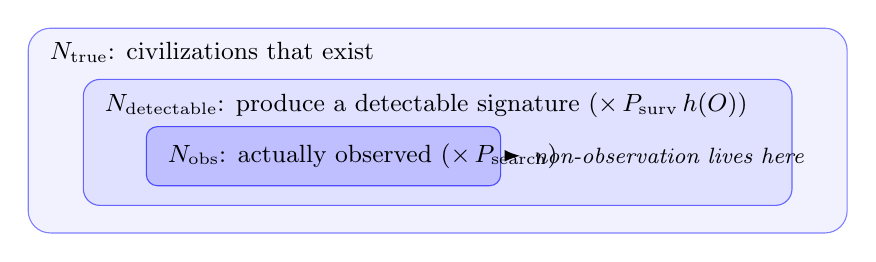
\begin{tikzpicture}[font=\small]
  \draw[rounded corners=8pt, fill=blue!5, draw=blue!50]
        (0,0) rectangle (10.4,2.6);
  \node[anchor=north west] at (0.15,2.55) {$\Ntrue$: civilizations that exist};
  \draw[rounded corners=6pt, fill=blue!12, draw=blue!60]
        (0.7,0.35) rectangle (9.7,1.95);
  \node[anchor=north west] at (0.85,1.9) {$\Ndet$: produce a detectable signature ($\times\,\Psurv\, h(\Obs)$)};
  \draw[rounded corners=4pt, fill=blue!25, draw=blue!70]
        (1.5,0.6) rectangle (6.0,1.35);
  \node[anchor=west] at (1.65,0.98) {$\Nobs$: actually observed ($\times\,\Psearch$)};
  \node[anchor=west, font=\itshape\footnotesize] at (6.3,0.98) {non-observation lives here};
  \draw[-{Latex[length=2mm]}, thick] (6.05,0.98) -- (6.25,0.98);
\end{tikzpicture}
\caption{Existence, detectability and observation are distinct. Non-observation
constrains the innermost set, and therefore only the \emph{product} of the
factors in Eq.~\eqref{eq:decomp}; it does not by itself constrain $\Ntrue$.}
\label{fig:venn}
\end{figure}

\begin{figure}[t]
\centering
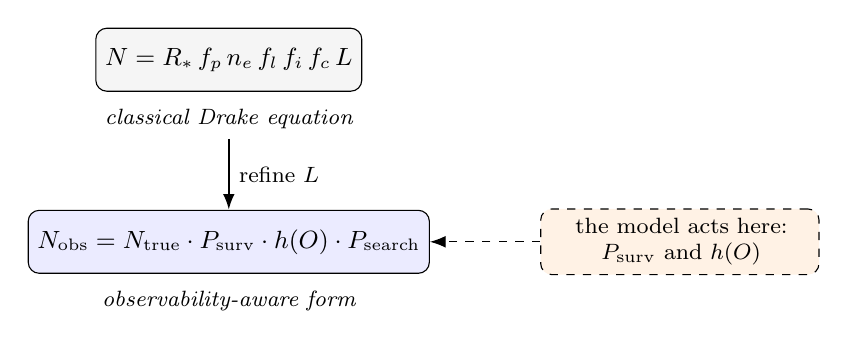
\begin{tikzpicture}[font=\small, node distance=3mm]
  \node (drake) [draw, rounded corners, fill=gray!8, minimum height=8mm]
    {$N = R_*\, f_p\, n_e\, f_l\, f_i\, f_c\, L$};
  \node (lab1) [below=1mm of drake, font=\footnotesize\itshape] {classical Drake equation};
  \node (arrow) [below=7mm of lab1] {};
  \node (rof) [draw, rounded corners, fill=blue!8, minimum height=8mm, below=9mm of lab1]
    {$\Nobs = \Ntrue \cdot \Psurv \cdot h(\Obs) \cdot \Psearch$};
  \node (lab2) [below=1mm of rof, font=\footnotesize\itshape] {observability-aware form};
  \draw[-{Latex[length=2mm]}, thick] (lab1) -- node[right, font=\footnotesize] {refine $L$} (rof);
  \node (act) [right=14mm of rof, draw, dashed, rounded corners, fill=orange!10,
               text width=3.3cm, align=center, font=\footnotesize]
    {the model acts here:\\ $\Psurv$ and $h(\Obs)$};
  \draw[-{Latex[length=2mm]}, dashed] (act) -- (rof);
\end{tikzpicture}
\caption{The framework is a refinement of the Drake equation's lifetime and
detectability content, not a replacement for it. It leaves the astrophysical
factors untouched and acts on survival and signal production.}
\label{fig:drakemap}
\end{figure}

\subsection{Why this matters for inference}

Suppose a survey reports no detections. Under Eq.~\eqref{eq:decomp} the
likelihood of that outcome depends on $\Psearch$ and on the distribution of
$\Obs$ across the population, not on $\Ntrue$ alone. Two very different worlds
--- one in which civilizations are rare, and one in which they are common but
mostly quiet during the epoch we can sample --- produce the same null result.
Distinguishing them requires a model of how $\Obs$ is distributed and how it
evolves, which is what \S\ref{sec:model} supplies. \Established

\subsection{What observability is, and is not}

We use $\Obs$ for \emph{external observability}: the strength of signatures
leaving the system, aggregating waste heat, leakage and intentional emission,
expansion footprint, and engineered structures. It is not energy use, and it is
not capability. A civilization may be extremely capable and comparatively quiet;
it may also be modest and loud.

Crucially, $\Obs$ can be small but never zero. Any energy use produces
thermodynamic consequences, and a claim of true invisibility would require
physics we have no warrant to assume \citep{dyson1960,kardashev1964}. We encode
this directly: $\Obs$ is bounded below by a strictly positive floor $\Ofloor$
(Proposition~\ref{prop:obs}). Low observability in this framework always means
``hard to detect'', never ``absent''. \Established

\section{The dynamical model}
\label{sec:model}

\subsection{Variables}

Three quantities evolve together in a dimensionless time $\tau$.

\begin{description}\itemsep3pt
  \item[$\Icap(\tau)$ --- effective capability.] A compressed systems variable
    that rolls together scientific capability, automation, computational
    capacity, coordination and technological leverage. It is not a measure of
    intelligence in the psychometric sense, not a measure of moral worth, and
    not a measure of consciousness. A civilization can grow enormously in
    $\Icap$ without becoming wiser, safer or louder.
  \item[$\Reg(\tau)$ --- regulatory capacity.] Alignment, governance, safety
    culture, institutional learning, epistemic reliability, error correction:
    whatever it takes to stop a runaway. We treat it as a \emph{quality index}
    normalised to $[0,1]$, and that normalisation is what makes it
    commensurable with the growth rates it has to oppose (\S\ref{sec:reg-eq}).
  \item[$\Obs(\tau)$ --- external observability.] Signature strength as defined
    in \S\ref{sec:decomp}, bounded below by $\Ofloor > 0$.
\end{description}

Table~\ref{tab:vars} lists these with their drivers. Figure~\ref{fig:ladder}
maps the usual civilizational stages onto them, and Figure~\ref{fig:schematic}
shows what is coupled to what.

\begin{table}[tb]
\centering\small
\caption{Model variables and drivers. The three states are integrated; the
drivers are exogenous inputs the user sets.}
\label{tab:vars}
\begin{tabular}{@{}llp{7.1cm}@{}}
\toprule
Symbol & Role & Interpretation \\
\midrule
$\Icap$   & state  & effective capability: science, automation, computation, coordination \\
$\Reg$    & state  & regulatory quality index in $[0,1]$: alignment, governance, error correction \\
$\Obs$    & state  & external observability: leakage, waste heat, expansion footprint \\
\midrule
$A$       & driver & ordinary amplification pressure (baseline technological leverage) \\
$\Arec$   & driver & recursive amplification: self-improvement, automated design, compute scaling \\
$\Aref$   & driver & reflective amplification: capability aimed at safety and foresight \\
$Q$       & driver & institutional quality \\
\bottomrule
\end{tabular}
\end{table}

\begin{figure}[tb]
\centering
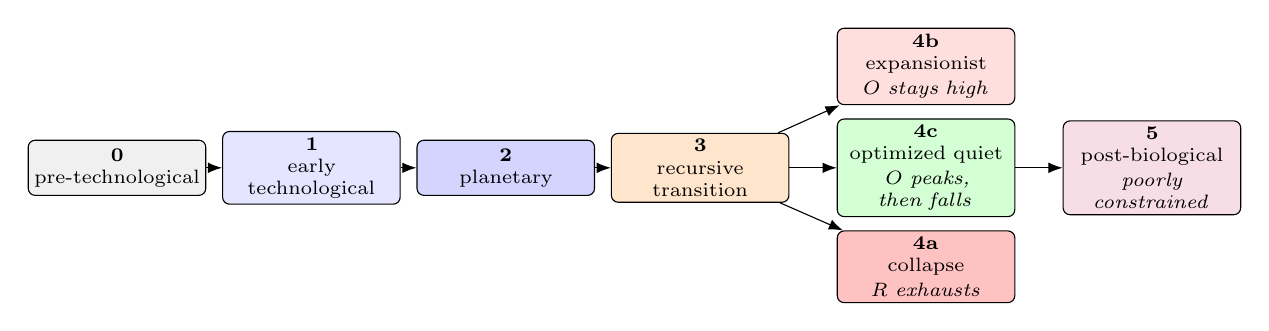
\begin{tikzpicture}[font=\scriptsize, >={Latex[length=1.8mm]}]
  % Algorithmic hyphenation off: these boxes are too narrow for it to look
  % like anything but a mistake.  Explicit hyphens may still break.
  \hyphenpenalty=10000
  \tikzset{stg/.style={draw, rounded corners=2.5pt, minimum height=7mm,
                       text width=2.1cm, align=center, inner sep=2.2pt,
                       fill=#1}}
  \node[stg=gray!12]                      (s0) {\textbf{0}\\pre-technological};
  \node[stg=blue!10,   right=2mm of s0]   (s1) {\textbf{1}\\early technological};
  \node[stg=blue!17,   right=2mm of s1]   (s2) {\textbf{2}\\planetary};
  \node[stg=orange!20, right=2mm of s2]   (s3) {\textbf{3}\\recursive transition};

  \node[stg=red!13,    above right=3.5mm and 6mm of s3] (s4b)
       {\textbf{4b}\\expansionist\\[1pt]\textit{$\Obs$ stays high}};
  \node[stg=green!17,  right=6mm of s3]                 (s4c)
       {\textbf{4c}\\optimized quiet\\[1pt]\textit{$\Obs$ peaks, then falls}};
  \node[stg=red!24,    below right=3.5mm and 6mm of s3] (s4a)
       {\textbf{4a}\\collapse\\[1pt]\textit{$\Reg$ exhausts}};
  \node[stg=purple!13, right=6mm of s4c]                (s5)
       {\textbf{5}\\post-biological\\[1pt]\textit{poorly constrained}};

  \draw[->] (s0)--(s1);  \draw[->] (s1)--(s2);  \draw[->] (s2)--(s3);
  \draw[->] (s3)--(s4b); \draw[->] (s3)--(s4c); \draw[->] (s3)--(s4a);
  \draw[->] (s4c)--(s5);
\end{tikzpicture}
\caption{Civilizational stages, and the branch at the recursive transition.
Stages 0--2 are pre-recursive and behave the way anyone would expect. Everything
interesting happens at stage~3, where the same machinery can go three different
ways depending on which term wins.}
\label{fig:ladder}
\end{figure}

\begin{figure}[tb]
\centering
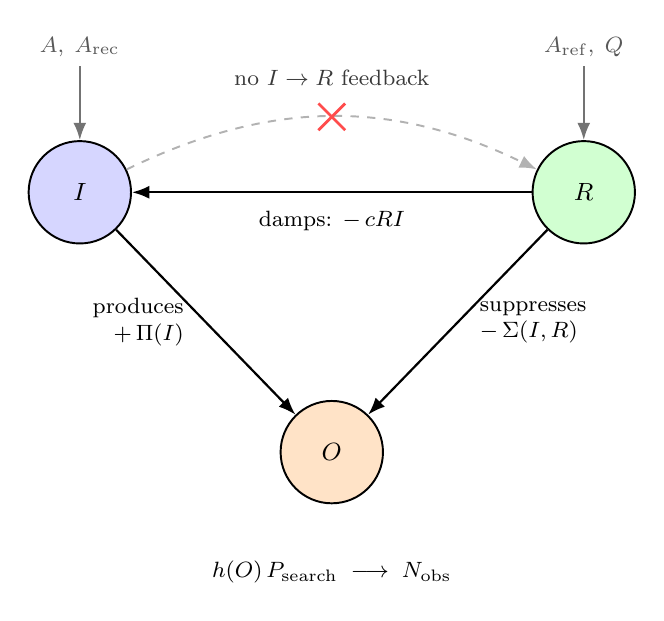
\begin{tikzpicture}[font=\small, >={Latex[length=2.2mm]}]
  \tikzset{var/.style={draw, circle, minimum size=13mm, line width=0.7pt, fill=#1},
           drv/.style={font=\footnotesize, align=center, text=black!65}}

  \node[var=blue!16]   (I) at (0,0)      {$\Icap$};
  \node[var=green!18]  (R) at (6.4,0)    {$\Reg$};
  \node[var=orange!22] (O) at (3.2,-3.3) {$\Obs$};

  % exogenous drivers feeding the two upper states
  \node[drv] (dI) at (0,1.85)   {$A,\;\Arec$};
  \node[drv] (dR) at (6.4,1.85) {$\Aref,\;Q$};
  \draw[->, thick, black!55] (dI) -- (I);
  \draw[->, thick, black!55] (dR) -- (R);

  % regulation damps capability
  \draw[->, thick] (R) -- (I);
  \node[anchor=north, font=\footnotesize, yshift=-1.2mm] at ($(I)!0.5!(R)$)
       {damps: $-\,c\Reg\Icap$};

  % the feedback that is deliberately absent -- drawn, then struck out
  \draw[->, dashed, gray!60, line width=0.7pt] (I) to[bend left=26]
        node[pos=0.5, inner sep=0] (nf) {} (R);
  \draw[red!70, line width=1pt] ($(nf)+(-1.7mm,-1.7mm)$) -- ($(nf)+(1.7mm,1.7mm)$);
  \draw[red!70, line width=1pt] ($(nf)+(-1.7mm,1.7mm)$) -- ($(nf)+(1.7mm,-1.7mm)$);
  \node[above=2.4mm of nf, font=\footnotesize, text=gray!45!black]
       {no $\Icap \rightarrow \Reg$ feedback};

  % production and suppression of the signature
  \draw[->, thick] (I) -- node[left, font=\footnotesize, align=right, xshift=-1.5mm]
       {produces\\$+\,\Pi(\Icap)$} (O);
  \draw[->, thick] (R) -- node[right, font=\footnotesize, align=left, xshift=1.5mm]
       {suppresses\\$-\,\Sigma(\Icap,\Reg)$} (O);

  \node[below=6mm of O, font=\footnotesize]
       {$h(\Obs)\,\Psearch \;\longrightarrow\; \Nobs$};
\end{tikzpicture}
\caption{What is coupled to what. Regulation damps capability through
$-c\Reg\Icap$. Observability is produced by capability and suppressed
fractionally by capability \emph{and} regulation acting together --- $\Sigma$
depends on both, even though the arrow has to be drawn from one of them. The
struck-out arc is the coupling this model does \emph{not} have: in
Eq.~\eqref{eq:dR}, regulatory capacity responds to the exogenous drivers and to
erosion by $\Arec$, but never to capability itself. Closing that loop is the
most interesting extension we can see (\S\ref{sec:limitations}).}
\label{fig:schematic}
\end{figure}

\subsection{Capability}

Capability grows two ways: by ordinary accumulation, $a A \Icap$, and by
recursive amplification, $b \Arec F(\Icap)$, where $F$ says how aggressive the
recursion is. It is held back by regulatory friction, $c \Reg \Icap$, and it
eventually runs into physical, energetic and coordination limits, $s_I \Icap^2$:
\begin{equation}
  \dd{\Icap}{\tau} \;=\; a A \Icap \;+\; b \Arec F(\Icap) \;-\; c \Reg \Icap \;-\; s_I \Icap^2 .
  \label{eq:dI}
\end{equation}
Every term is there because some mechanism puts it there. That is the point: the
equation is assembled out of balances you can argue with, not written down
because it integrates nicely.

\subsection{Regulation}
\label{sec:reg-eq}

Regulatory capacity is built by reflective capability and institutional quality,
and eroded by the sheer pace of recursive amplification. The modelling choice
that matters is this: erosion has to be proportional to the regulation that is
actually there, because you cannot erode capacity that does not exist, and
building has to act on whatever headroom is left. So
\begin{equation}
  \dd{\Reg}{\tau} \;=\; \underbrace{(u \Aref + v Q)}_{\textstyle B}\,(1-\Reg)
                 \;-\; \underbrace{(w \Arec + s_R)}_{\textstyle W}\,\Reg .
  \label{eq:dR}
\end{equation}

\begin{proposition}[Regulation is confined to the unit interval]
\label{prop:reg}
If $B \geq 0$ and $W \geq 0$ and $\Reg(0) \in [0,1]$, then $\Reg(\tau) \in [0,1]$
for all $\tau > 0$, and
\begin{equation}
  \Reg_\infty = \frac{B}{B+W} = \frac{u \Aref + v Q}{u \Aref + v Q + w \Arec + s_R} .
  \label{eq:Rinf}
\end{equation}
\end{proposition}

\begin{proof}
At $\Reg = 0$, Eq.~\eqref{eq:dR} gives $\mathrm{d}\Reg/\mathrm{d}\tau = B \geq 0$,
so the lower boundary cannot be crossed downwards. At $\Reg = 1$ it gives
$\mathrm{d}\Reg/\mathrm{d}\tau = -W \leq 0$, so the upper boundary cannot be
crossed upwards. With constant drivers Eq.~\eqref{eq:dR} is linear in $\Reg$,
$\mathrm{d}\Reg/\mathrm{d}\tau = B - (B+W)\Reg$, which gives the stated fixed
point and $\Reg(\tau)=\Reg_\infty+(\Reg_0-\Reg_\infty)e^{-(B+W)\tau}$.
\end{proof}

Two things follow, and both are worth pausing on. First, $\Reg_\infty$ is a
\emph{share}: the fraction of the total pressure on governance that happens to
be constructive. That makes it something you can reason about directly. Second,
because $\Reg$ can never go negative, the damping term $-c\Reg\Icap$ in
Eq.~\eqref{eq:dI} can never flip sign. Let $\Reg$ go negative and failing
governance starts \emph{accelerating} capability, which is not a mechanism
anybody means to model --- it is an arithmetic accident wearing a mechanism's
clothes.

\subsection{Observability}

Observability is produced by energy use, broadcast leakage and expansion
footprint, and suppressed by compression and stealth. The suppression is
fractional: it acts on the signal actually being emitted, above an irreducible
floor.
\begin{equation}
  \dd{\Obs}{\tau} \;=\; \underbrace{p E(\Icap) + q B_{\mathrm c}(\Icap) + r X(\Icap)}_{\textstyle \Pi(\Icap)}
  \;-\; (\Obs - \Ofloor)\,\underbrace{\big(m C(\Icap,\Reg) + n S(\Icap,\Reg)\big)}_{\textstyle \Sigma(\Icap,\Reg)} .
  \label{eq:dO}
\end{equation}

\begin{proposition}[Observability is bounded below by the floor]
\label{prop:obs}
If $\Pi \geq 0$ and $\Sigma \geq 0$ and $\Obs(0) \geq \Ofloor$, then
$\Obs(\tau) \geq \Ofloor$ for all $\tau > 0$. Where $\Sigma > 0$, the
quasi-steady observability is
\begin{equation}
  \Obs^{*} \;=\; \Ofloor + \frac{\Pi(\Icap)}{\Sigma(\Icap,\Reg)} .
  \label{eq:Ostar}
\end{equation}
\end{proposition}

\begin{proof}
At $\Obs = \Ofloor$ the suppression term vanishes identically, leaving
$\mathrm{d}\Obs/\mathrm{d}\tau = \Pi \geq 0$, so the floor cannot be crossed
downwards. Setting $\mathrm{d}\Obs/\mathrm{d}\tau = 0$ in Eq.~\eqref{eq:dO} and
solving for $\Obs$ gives Eq.~\eqref{eq:Ostar}.
\end{proof}

Equation~\eqref{eq:Ostar} is the analytical heart of this paper, and the reason
is that $\Obs^{*}$ is a \emph{ratio}. What it does as capability grows is
decided by how production and suppression scale \emph{against each other},
never by either one alone:
\begin{equation}
  \Pi \sim \Icap, \quad \Sigma \sim \Icap \Reg
    \;\Longrightarrow\; \Obs^{*} \sim \frac{1}{\Reg}
    \qquad\text{(observability independent of capability)},
\end{equation}
\begin{equation}
  \Pi \sim \Icap, \quad \Sigma \sim \Icap^{2} \Reg
    \;\Longrightarrow\; \Obs^{*} \sim \frac{1}{\Icap \Reg}
    \qquad\text{(observability declines with capability)}.
  \label{eq:decline}
\end{equation}
Look at what the second line does. It produces peak-then-decline without anyone
choosing a peaked function --- the shape falls out of the ratio. That is what we
mean by the signature being derived rather than assumed, and \S\ref{sec:results}
shows it happening numerically. \Plausible

\subsection{Interchangeable functional forms}

None of the functional forms above is privileged, and we would rather not
pretend otherwise. Each is drawn from a registry (Table~\ref{tab:registry}), so
asking whether a conclusion survives a change of functions is a menu selection
instead of a rewrite. That is what turns robustness from an aspiration into
something you can actually check in an afternoon.

\begin{table}[tb]
\centering\small
\caption{Interchangeable functional forms. Any combination is admissible; the
solver never refers to a specific choice.}
\label{tab:registry}
\begin{tabular}{@{}lL{3.3cm}L{6.6cm}@{}}
\toprule
Component & Variants & Form \\
\midrule
$F(\Icap)$ recursion & linear, superlinear, Lambert, exponential, saturating &
  $\Icap$; $\Icap^2$; $\Icap e^{\Icap}$; $e^{\Icap}$; $\Icap/(1+\Icap/K)$ \\
$\Obs(\Icap)$ static & A increasing, B decreasing, C peaked, D threshold &
  $1-e^{-\lambda \Icap}$; $e^{-\lambda \Icap}$; $\Icap e^{-\lambda \Icap}$; $\sigma\!\big(k(\Icap-\Icap_c)\big)$ \\
$E$ energy use & linear, Kardashev & $\Icap$; $\Icap^2$ \\
$B_{\mathrm c}$ broadcast & linear, decaying & $\Icap$; $\Icap e^{-\lambda \Icap}$ \\
$X$ expansion & linear, inward & $\Icap$; $0$ \\
$C$, $S$ suppression & linear, superlinear & $\Icap \Reg$; $\Icap^{2}\Reg$ \\
\bottomrule
\end{tabular}
\end{table}

\subsection{Regime classification}

Trajectories are labelled by the criteria in Table~\ref{tab:regimes}, checked in
a fixed order. The order is not commutative --- a trajectory that meets two
criteria gets the earlier label --- and we say so explicitly because it changes
how the phase portrait in \S\ref{sec:results} should be read.

\begin{table}[tb]
\centering\small
\caption{Regime criteria, in evaluation order. Thresholds are model parameters,
not empirical quantities.}
\label{tab:regimes}
\begin{tabular}{@{}llL{6.4cm}l@{}}
\toprule
\# & Regime & Criterion & Strength \\
\midrule
1 & collapse proxy & runaway \emph{and} ($\Reg<\Rmin$ or $\Obs$ peaked then fell below $\Odet$) & \Hypothetical \\
2 & runaway & $\Icap>I_{\mathrm{runaway}}$ or $\Arec/(\Reg+\epsilon)>\Theta$ & \Speculative \\
3 & pre-detectable & $\max\Obs<\Odet$ and $\max\Icap<\Iadv$ & \Plausible \\
4 & optimized low-observable & $\Icap\geq\Iadv$, $\Reg\geq\Rmin$, $\Obs<\Odet$ & \Hypothetical \\
5 & expansionist visible & $\Icap\geq\Iadv$ and $\Obs\geq\Odet$ & \Hypothetical \\
6 & visible technological & $\Pdet>0.01$ & \Plausible \\
7 & uncertain & none of the above & \Plausible \\
\bottomrule
\end{tabular}
\end{table}

Regime~1 is called a \emph{proxy} on purpose. There is no mortality term
anywhere in this model, so what it registers is the conditions under which
collapse should be expected --- not a collapse. We come back to this in
\S\ref{sec:limitations}, because it is a real limitation and not a quibble.

\section{The Lambert threshold, and why it is auxiliary}
\label{sec:lambert}

This section reports a negative result about our own starting point.

The Lambert $W$ function motivated the original formulation of this work, and it
is mathematically correct everywhere we use it. But the balance that justifies
$W$ turns out not to be the balance governing the system we actually integrate.
We could have quietly kept the boundary and let it look like a property of the
dynamics. We would rather set the whole thing out, because noticing this kind of
gap is exactly what separates a model you can use from mathematics you can
admire.

\subsection{When $W$ is actually required}

The Lambert $W$ function is defined implicitly by $W(y)e^{W(y)} = y$, and you
need it precisely when an unknown shows up both inside and outside an
exponential \citep{corless1996}. A relation
\begin{equation}
  x e^{x} = y \quad\Longrightarrow\quad x = W(y)
\end{equation}
genuinely requires it. A relation $e^{x} = y$ does not; that is a logarithm. Any
appearance of $W$ that does not rest on the first structure is decoration.

\subsection{The natural balance does not need $W$}

Take the Lambert recursion kernel $F(\Icap) = \Icap e^{\Icap}$ from
Table~\ref{tab:registry}. Equation~\eqref{eq:dI} becomes
\begin{equation}
  \dd{\Icap}{\tau} = a A \Icap + b \Arec \Icap e^{\Icap} - c \Reg \Icap - s_I \Icap^{2}.
\end{equation}
Set recursive amplification against regulatory damping, drop ordinary growth and
saturation for the moment, and you get
\begin{equation}
  b \Arec \Icap e^{\Icap} \;=\; c \Reg \Icap .
\end{equation}
Now look at what happens. For $\Icap > 0$ the factor $\Icap$ \emph{cancels on
both sides}, and we are left with
\begin{equation}
  b \Arec e^{\Icap} = c \Reg
  \qquad\Longrightarrow\qquad
  \Icap_{\mathrm{thr}} = \ln\!\left(\frac{c \Reg}{b \Arec}\right),
  \label{eq:logthreshold}
\end{equation}
a \emph{logarithmic} threshold. The Lambert structure is destroyed by the very
cancellation that the $\Icap e^{\Icap}$ kernel appeared to guarantee. The
damping term carries a factor of $\Icap$ too, and the two factors annihilate.
This is the central observation of the section, and it is remarkably easy to
miss --- we missed it for a while.

\subsection{Recovering Lambert structure requires a different balance}

Lambert structure survives only if $\Icap e^{\Icap}$ is set against a regulatory
capacity that is \emph{not} itself proportional to $\Icap$. Introduce such a
capacity,
\begin{equation}
  C_R \;=\; c\,\Reg^{\eta}\,\ln(1 + \Aref)\,\mathcal{E},
  \label{eq:CR}
\end{equation}
with $\eta$ a regulation exponent and $\mathcal{E}$ an alignment factor, impose
$b \Arec \Icap e^{\Icap} = C_R$, and now nothing cancels:
\begin{equation}
  \Icap e^{\Icap} = \frac{C_R}{b \Arec}
  \qquad\Longrightarrow\qquad
  \boxed{\;\Icrit \;=\; W\!\left(\frac{c\,\Reg^{\eta}\,\ln(1+\Aref)\,\mathcal{E}}{b \Arec}\right).}
  \label{eq:Icrit}
\end{equation}
Equation~\eqref{eq:Icrit} is a clean Lambert boundary, and it is what
Figure~\ref{fig:lambert} shows.

\subsection{The honest reading}

Here is the difficulty. $C_R$ appears nowhere in Eq.~\eqref{eq:dI}. The system we
integrate contains the damping term $-c\Reg\Icap$, whose threshold is
Eq.~\eqref{eq:logthreshold} --- logarithmic. So Eq.~\eqref{eq:Icrit} describes a
balance we have \emph{posited alongside} the dynamics, not one the dynamics
contain. Stating it plainly:

\begin{quote}
The Lambert boundary $\Icrit = W(C_R / b\Arec)$ is an \emph{auxiliary stability
diagnostic} evaluated under a stated auxiliary balance. It is not a bifurcation
of the integrated system, and no result in \S\ref{sec:results} depends on it.
\Hypothetical
\end{quote}

The implementation enforces that distinction rather than trusting the prose to
carry it: the Lambert branch is guarded so $W$ is evaluated only when the
Lambert kernel is genuinely selected, and every other kernel falls back to the
logarithmic threshold of Eq.~\eqref{eq:logthreshold}. Verification of the
identity $\Icrit e^{\Icrit} = C_R/(b\Arec)$ to machine precision is reported in
\S\ref{sec:verification}.

\begin{figure}[tb]
\centering
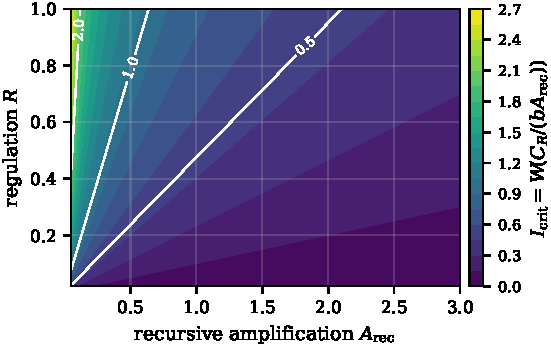
\includegraphics[width=\textwidth]{figures/fig09_lambert_boundary.pdf}
\caption{The auxiliary Lambert boundary $\Icrit$ against recursive amplification,
at five fixed values of regulatory capacity, from Eq.~\eqref{eq:Icrit}. More
regulation raises the critical capability that can be absorbed; stronger
recursive amplification lowers it, and does so steeply at small $\Arec$. This is
a diagnostic evaluated under the auxiliary balance of Eq.~\eqref{eq:CR}, not a
bifurcation set of the integrated system.}
\label{fig:lambert}
\end{figure}

\subsection{Why keep it at all}

Three reasons. It gives an analytic handle on the intuition that regulation can
only absorb so much recursive amplification. It makes the comparison between
regulatory capacity and amplification pressure explicit and plottable. And,
reported honestly, it is a worked example of the discipline the rest of the
framework demands: a candidate piece of mathematics, tested to see whether it was
really required, and found to be required only under an assumption we then have
to declare out loud.

\section{Numerical methods and verification}
\label{sec:verification}

Models of this kind are rarely verified beyond ``the code runs and the plots look
plausible''. Because the conclusions here depend on the qualitative shape of
computed trajectories, we treat verification as a first-class part of the
contribution and report it in full.

\subsection{Integration}

The system \eqref{eq:dI}--\eqref{eq:dO} is integrated with an explicit adaptive
Dormand--Prince Runge--Kutta method of order 5(4) with dense output
\citep{dormand1980}, as provided by SciPy \citep{virtanen2020scipy,harris2020numpy},
at relative tolerance $10^{-6}$ and absolute tolerance $10^{-9}$. All
exponentials are argument-clipped to $[-50,50]$ to prevent overflow.

Two of the recursion kernels in Table~\ref{tab:registry} --- superlinear and
exponential --- produce genuine finite-time blow-up, where $\Icap$ diverges at a
finite $\tau$. An adaptive stepper approaching such a singularity takes
ever-smaller steps and does not terminate. Integration therefore stops on a
terminal event when $\Icap$ exceeds a bound $I_{\mathrm{abort}}$ set two orders
of magnitude above the runaway threshold, and the remaining output samples hold
the terminal state. We note that padding instead with the last \emph{output}
sample is misleading: the singularity generally falls between samples, so the
recorded maximum can understate a divergence by orders of magnitude.

\subsection{Six independent oracles}

Each check below tests the implementation against something other than itself.
Results are summarised in Table~\ref{tab:verification}.

\paragraph{A. Closed-form regulation.}
Equation~\eqref{eq:dR} is linear in $\Reg$ and --- importantly --- independent of
$\Icap$ and $\Obs$. It therefore integrates exactly, giving
$\Reg(\tau)=\Reg_\infty+(\Reg_0-\Reg_\infty)e^{-(B+W)\tau}$ with $\Reg_\infty$
from Eq.~\eqref{eq:Rinf}. Every configuration reproduces this to
$\leq 2.3\times10^{-6}$, consistent with the requested tolerance.

\paragraph{B. Independent high-order integrator.}
Every configuration was re-integrated with an eighth-order Dormand--Prince method
at tolerances $10^{-12}/10^{-14}$ and compared against the production solver at
its default settings. All twenty agree. For the two blow-up kernels the
comparison is restricted to the interval before the abort event, since the
reference has no such guard.

\paragraph{C. Independent quadrature of the observability equation.}
$\mathrm{d}\Obs/\mathrm{d}\tau$ was reconstructed from the computed $\Icap,\Reg$
and integrated by quadrature, independently of the ODE solver's treatment of
$\Obs$. Agreement is $\leq 1.5\times10^{-4}$ on all non-singular configurations.

\paragraph{D. The Lambert identity.}
$\Icrit$ must satisfy its own definition, $\Icrit e^{\Icrit} = C_R/(b\Arec)$.
Across 576 parameter combinations and four values of $\Reg$ --- 2304 evaluations
--- the maximum relative residual is $4.4\times10^{-16}$, i.e.\ machine
precision. The validity guard also behaves as specified, returning no boundary
for any non-Lambert kernel.

\paragraph{E. Property-based invariant testing.}
Propositions~\ref{prop:reg} and~\ref{prop:obs} assert structural bounds, so they
should hold for \emph{arbitrary} admissible parameters rather than for tuned
presets. Three hundred randomised parameter sets were drawn across the full
declared ranges, with randomised recursion kernels and suppression forms. There
were \textbf{no violations}: the global minimum observability was
$2.16\times10^{-3}$, above the floor, and regulation remained within
$[4.0\times10^{-3},\,0.999]$. This is the strongest single piece of evidence that
the bounds are structural and not artefacts of parameter choice.

\paragraph{F. Two independent implementations.}
The model is implemented twice: once in Python against SciPy, and once in
JavaScript with a separately written adaptive Dormand--Prince integrator,
its own dense-output interpolation, its own initial-step heuristic, and a
hand-implemented Lambert $W_0$ via Halley iteration. Across the twenty
configurations the worst absolute discrepancies are
$|\Delta \Icap| = 5.2\times10^{-5}$,
$|\Delta \Reg| = 3.1\times10^{-7}$ and
$|\Delta \Obs| = 2.7\times10^{-5}$; $\Icrit$ agrees to $2.2\times10^{-12}$
relative; and \emph{all twenty regime classifications are identical}.
Figure~\ref{fig:crossval} shows the comparison with residuals.

The independent $W_0$ implementation was itself checked against the defining
identity over $x\in[10^{-6},10^{6}]$ and across the negative branch
$x\in[-1/e,0)$, with maximum relative residual $1.0\times10^{-15}$.

\begin{table}[t]
\centering\small
\caption{Verification results. Each oracle tests the implementation against
something other than itself.}
\label{tab:verification}
\begin{tabular}{@{}clll@{}}
\toprule
 & Oracle & Scope & Result \\
\midrule
A & closed-form $\Reg(\tau)$              & 19 configurations & max error $2.3\times10^{-6}$ \\
B & independent 8th-order integrator      & 20 configurations & 20/20 agree \\
C & quadrature of $\mathrm{d}\Obs/\mathrm{d}\tau$ & 12 non-singular configurations & $\leq 1.5\times10^{-4}$ \\
D & Lambert identity                      & 2304 evaluations  & $4.4\times10^{-16}$ \\
E & structural invariants                 & 300 random configurations & \textbf{0 violations} \\
F & Python vs.\ JavaScript                & 20 configurations & $|\Delta \Icap|=5.2\times10^{-5}$; labels identical \\
\bottomrule
\end{tabular}
\end{table}

\begin{figure}[t]
\centering
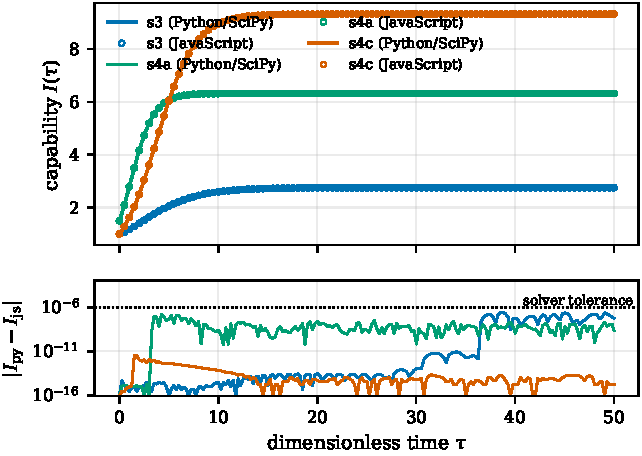
\includegraphics{figures/fig10_cross_validation.pdf}
\caption{Cross-validation of two independent implementations. Upper: capability
trajectories for three stages, Python (lines) and JavaScript (markers). Lower:
absolute difference, which stays at or below the requested solver tolerance
across the integration. The two codes share no numerical machinery.}
\label{fig:crossval}
\end{figure}

\subsection{What verification does and does not establish}

These checks establish that the equations we describe are the equations being
solved, and that they are solved accurately. They say nothing about whether the
equations describe a real civilization: no term here has been calibrated against
data, because no relevant data exist. The distinction between a verified model
and a validated one is worth keeping sharp, and we make no claim to the latter.
\Established

\section{Results}
\label{sec:results}

Everything below uses the parameter set in Appendix~\ref{app:params}, and every
number can be reproduced from the simulator.

\subsection{Stage trajectories}

Figure~\ref{fig:stages} shows capability, regulation and observability for the
eight canonical stage configurations. Table~\ref{tab:stagecheck} sets what each
stage actually did against what that stage is \emph{defined} to do. This is a
low bar, and we report it because it is a bar models fail all the time without
anyone noticing --- a stage called ``collapse'' that quietly grows is the sort
of thing that survives for years inside a plausible-looking plot.

Two configurations reward a closer look. Stage~1, the early technological
phase, has no regulatory damping at all, so capability reduces to a plain
logistic equation and hits its analytic limits exactly: $\Icap \to aA/s_I = 3.0$
and $\Obs \to 1-e^{-\lambda \Icap} = 0.5934$ (Appendix~\ref{app:closed}).
Stage~4a drives regulation down to $\Reg_\infty = 0.0438$, below the collapse
threshold $\Rmin=0.05$ --- and it gets there \emph{without $\Reg$ ever going
negative}. Collapse happens by regulatory exhaustion, the mechanism we meant to
model, rather than by a sign flip in the damping term, which is the mechanism we
did not.

\begin{figure}[tb]
\centering
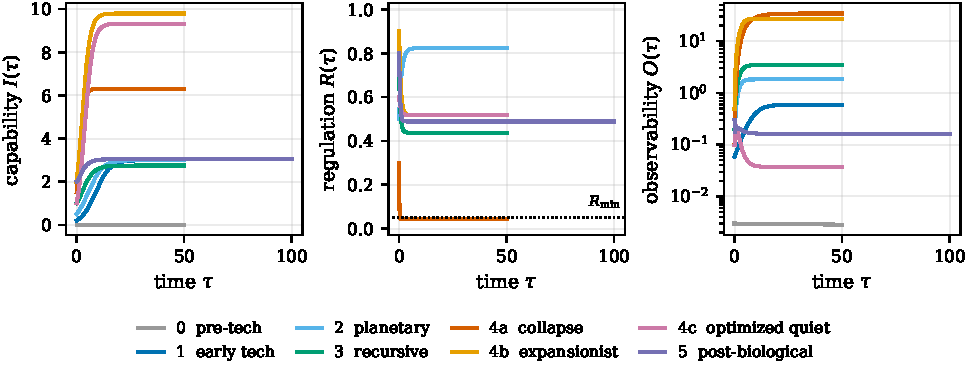
\includegraphics[width=\textwidth]{figures/fig05_stage_trajectories.pdf}
\caption{Capability, regulation and observability across the eight stage
configurations. Regulation stays inside $[0,1]$ by
Proposition~\ref{prop:reg}. Observability is plotted logarithmically and stays
strictly positive by Proposition~\ref{prop:obs}, spanning nearly five orders of
magnitude from the quietest stage to the loudest.}
\label{fig:stages}
\end{figure}

\begin{table}[tb]
\centering\small
\caption{What each stage was specified to do, against what it did.}
\label{tab:stagecheck}
\begin{tabular}{@{}llll@{}}
\toprule
Stage & Specified behaviour & Simulated & Regime \\
\midrule
0   & $\mathrm{d}\Icap/\mathrm{d}\tau\approx0$, no signature & $\Icap=0.010$, $\Obs=0.003$ & pre-detectable \\
1   & $\Icap\to aA/s_I$, $\Obs$ rising & $\Icap=3.0000$, $\Obs=0.5934$ & visible technological \\
2   & capability grows, $\Obs$ still rising & $\Icap=3.000$, $\Obs:0.10\to1.82$ & visible technological \\
3   & full model, recursion active & $\Icap=2.75$, $\Obs=3.43$ & visible technological \\
4a  & regulation collapses & $\Reg\to0.0438<\Rmin$, $\Reg\geq0$ & collapse proxy \\
4b  & high $\Icap$, high $\Obs$ sustained & $\Icap=9.80$, $\Obs=27.0$ & expansionist visible \\
4c  & $\Obs$ peaks, then declines & $0.100\to0.231\to0.037$ & optimized low-observable \\
5   & speculative & $\Icap=3.04$, $\Obs:0.30\to0.16$ & visible technological \\
\bottomrule
\end{tabular}
\end{table}

\subsection{Peak-then-decline is derived, not imposed}
\label{sec:derived}

This is the central result, and Figure~\ref{fig:suppression} is the whole
argument in one picture. Both panels are the \emph{same} stage-4c
configuration. Only the form of the suppression term differs.

Panel (a) uses an absolute suppression term, $-mC-nS$, whose rate does not
depend on $\Obs$ at all. Observability passes through zero at $\tau\approx0.3$
and then just keeps going, reaching $-1431$ by the end of the run. And here is
the part that should bother you: under the criteria of Table~\ref{tab:regimes}
that trajectory is still labelled ``optimized low-observable'', because the
classifier looks at $\Obs < \Odet$ and finds it satisfied. The label is
arithmetically correct and physically empty. The civilization is not quiet. It
has fallen off the bottom of the model.

Panel (b) uses the fractional form of Eq.~\eqref{eq:dO}. Observability rises
from $0.100$ to a peak of $0.231$ at $\tau=0.65$, then decays to $0.037$: below
the detection threshold, above the thermodynamic floor, and strictly positive
the entire time.

Now, why does it decline? Nothing in this configuration picks a peaked
functional form --- $\Obs$ is integrated, not evaluated from some curve we chose
in advance. The decline comes straight out of Eq.~\eqref{eq:decline}.
Compression and stealth scale as $\Icap^{2}\Reg$ while production scales as
$\Icap$, so the quasi-steady observability $\Obs^{*} \sim 1/(\Icap\Reg)$ has to
fall as capability grows. The civilization gets harder to see because its
efficiency outruns its output. That is a mechanism, not a stipulation.
\Plausible

The distinction is the whole answer to the standing objection against
low-observability accounts of the Great Silence --- that they assume the very
thing they set out to explain. A model that selects a peaked $\Obs(\Icap)$ does
assume it, and the objection lands. A model that gets the peak out of the ratio
of two independently motivated terms does not, and has to be attacked somewhere
else: on whether the required scaling separation is physically plausible. We
think that is a much better argument to be having.

\begin{figure}[tb]
\centering
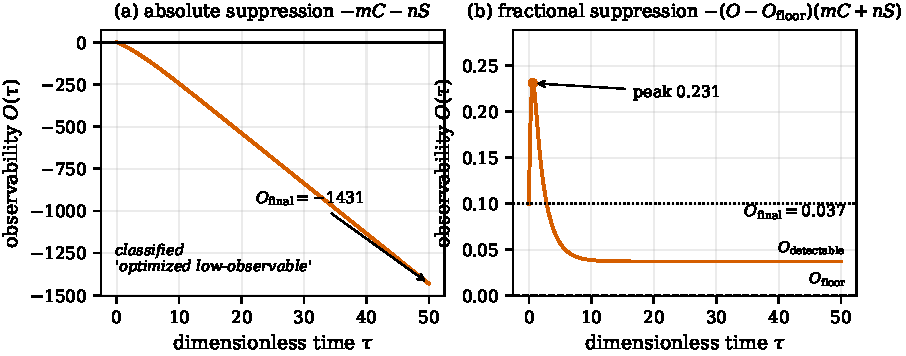
\includegraphics[width=\textwidth]{figures/fig07_suppression_comparison.pdf}
\caption{Why the form of the suppression term decides everything. Both panels
are the same configuration. (a) With absolute suppression the trajectory passes
through zero and dives, spending the entire run inside the shaded region the
model's own thermodynamics forbid --- and it is \emph{still} classified
``optimized low-observable''. (b) With fractional suppression and a
thermodynamic floor, the same configuration gives a genuine peak-then-decline,
bounded below. The decline is derived from suppression outscaling production,
not imposed by choosing a peaked profile.}
\label{fig:suppression}
\end{figure}

\subsection{Robustness across observability models}

Figure~\ref{fig:obsmodels} shows the four static observability models from
Table~\ref{tab:registry}: one rising, one falling, one peaked, one switching on
at a threshold. The framework admits all four.

The useful robustness question is not which curve is right. Nobody knows which
curve is right. The question is whether a conclusion survives changing it. The
low-observability regime is reachable under the peaked and decreasing models and
under the dynamical form of Eq.~\eqref{eq:dO}. It is \emph{not} reachable under
the increasing model, which instead gives the expansionist-visible regime we see
in stage~4b.

We count that as the framework working correctly. A model in which every
functional choice led to the same conclusion would not be testing anything at
all; it would be a machine for producing the answer we already had.
\Established

\begin{figure}[tb]
\centering
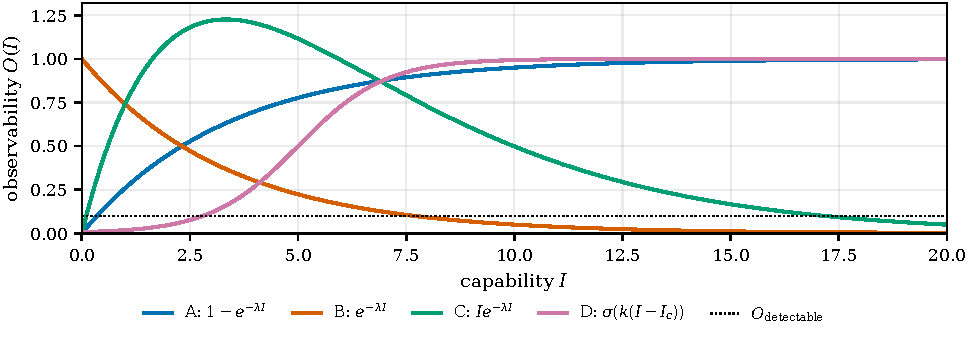
\includegraphics[width=\textwidth]{figures/fig06_observability_models.pdf}
\caption{The four interchangeable static observability models: A rises and
saturates, B falls from the start, C rises then falls, D switches on at a
threshold. Any conclusion about the Great Silence has to be reported together
with the model that produced it --- the low-observability regime does not arise
under model~A at all.}
\label{fig:obsmodels}
\end{figure}

\subsection{Phase structure}

Figure~\ref{fig:phase} puts the trajectories in the $(\Icap,\Reg)$ plane.
Because regulation is confined to $[0,1]$, the reachable phase space is a
bounded strip rather than a half-plane, and that makes the regime boundaries
directly readable off the picture: the vertical line at $\Iadv$ separates
pre-advanced from advanced capability, and the horizontal line at $\Rmin$ marks
regulatory exhaustion.

The branch structure of Figure~\ref{fig:ladder} is visible here as geometry.
Configurations that start in the same place separate according to whether
regulation holds: those keeping $\Reg\gtrsim0.5$ run to the right along the
strip into the advanced regimes, while stage~4a drops to the lower boundary and
trips the collapse proxy. \Hypothetical

\begin{figure}[tb]
\centering
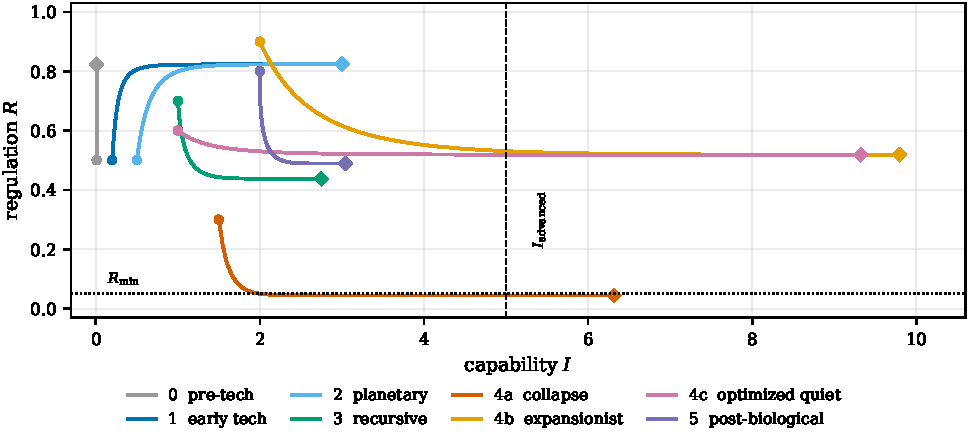
\includegraphics[width=\textwidth]{figures/fig08_phase_portrait.pdf}
\caption{Phase portrait in the capability--regulation plane. Circles mark
initial conditions, diamonds mark final states. Regulation is bounded to
$[0,1]$, so the reachable region is a strip, and the collapse boundary $\Rmin$
is approached but never crossed into negative values.}
\label{fig:phase}
\end{figure}

\subsection{Decomposing the silence}

Finally, Eq.~\eqref{eq:decomp} lets us ask which factor a null result actually
constrains. Take stage~4c, with $\Obs=0.037$, $\kappa=1$ and $\Psearch=0.5$. The
detection probability for a single civilization is
\begin{equation}
  \Pdet = \big(1-e^{-\kappa \Obs}\big)\Psearch = 0.018 ,
\end{equation}
against $\Pdet = 0.50$ for the expansionist stage~4b at $\Obs=27$. So the same
underlying population is about 27 times less likely to be detected in the quiet
regime than in the loud one --- with no change in $\Ntrue$ whatsoever, and
nobody going extinct. \Hypothetical

We want to be careful about what this does not show. It does not show that
civilizations are quiet, and it certainly does not show that quietness explains
the Great Silence. What it shows is narrower and, we think, more useful: under
this framework a null result is compatible with a wide range of $\Ntrue$, so
anyone attributing non-detection to rarity is making an argument about $\Obs$
and $\Psearch$ whether they say so or not. Usually they do not say so.

\section{Discussion}
\label{sec:discussion}

\subsection{Relation to existing solution classes}

The framework is not a rival to the standard families of Fermi-paradox
explanations but a way of expressing several of them in a common state space.

\paragraph{Great Filter.} A filter is a statement about where probability mass is
lost. In this framework a filter ahead of us appears as a region of parameter
space from which trajectories reach the collapse proxy --- and the model makes
explicit that a filter acting on \emph{observability} rather than survival is
also possible, and would be empirically indistinguishable from a survival filter
using non-detection alone \citep{hanson1998filter,cirkovic2018}. \Hypothetical

\paragraph{Grabby aliens.} \citet{hanson2021grabby} argue that if loud, expanding
civilizations explain human earliness, then quiet civilizations must also be
rare. This is the sharpest challenge to any low-observability account, ours
included, and we do not claim to answer it. What the framework contributes is a
place to state the disagreement precisely: the grabby-aliens argument constrains
the \emph{joint} distribution of expansion behaviour and timing, which in our
terms is a constraint on the population distribution of the expansion term $X$
and the branch probabilities at stage~3 --- quantities the present model takes
as given rather than derives. Coupling the two is the obvious next step.

\paragraph{Zoo and non-interference hypotheses.} These correspond to a stealth
term $S$ that is large and deliberate \citep{ball1973zoo,bracewell1960}. The
framework accommodates them but cannot distinguish deliberate quietness from
emergent efficiency, since both enter $\Sigma$ identically. That degeneracy is
worth stating: behavioural and thermodynamic explanations of quietness are not
separable by observability alone.

\paragraph{Percolation and expansion limits.} Models in which settlement stalls
\citep{landis1998,forgan2009,armstrong2013} act on $X$, the expansion
contribution to production, and are compatible with the ``inward'' variant in
Table~\ref{tab:registry}.

\subsection{Thermodynamic discipline}

The floor $\Ofloor$ is not a numerical convenience. Any civilization using energy
radiates, and the possibility of true invisibility would require assumptions we
have no basis to make \citep{dyson1960,kardashev1964}. Building the floor into
the equation rather than into the prose has a practical benefit: it makes the
strong claim unavailable. One cannot accidentally conclude from this model that
a civilization vanished, only that it became hard to detect at a stated
sensitivity $\kappa$ and coverage $\Psearch$. \Established

This is the substantive difference between the corrected and uncorrected
formulations of \S\ref{sec:derived}. The uncorrected version permitted arbitrarily
negative observability, and therefore permitted --- indeed produced --- a
conclusion that the framework's own thermodynamic commitments forbid.

\subsection{Implications for search strategy}

If the low-observability regime is populated at all, it has a testable
consequence. In that regime production is dominated by residual energy use
rather than by broadcast or expansion, since it is precisely the directed and
efficient channels that suppression acts on most strongly. Search programmes
sensitive to waste heat and infrared excess would then retain sensitivity where
narrowband beacon searches lose it \citep{dyson1960,wright2014ghat,garrett2015}.

This is a conditional, not a recommendation: it holds if C2 holds, and C2 is
labelled \Hypothetical. Its value is that it is the kind of statement that could
be wrong. Sustained null results from infrared surveys at improving sensitivity
would push against it \citep{griffith2015,wright2022haystack}.

\subsection{On the role of recursive and quantum capability}

The model treats $\Arec$ as an exogenous driver and does not explain where
recursive capability comes from. Quantum computation enters only as one possible
contributor to that driver --- a mechanism by which the simulation, search and
optimisation problems gating technological progress might be accelerated
\citep{shor1994,preskill2018}. We attach no magnitude to this and note that its
sign of effect on \emph{observability} is not determined: faster capability growth
raises production through $E$ and $\Icap$, but also raises suppression through
$C$ and $S$, and Eq.~\eqref{eq:Ostar} shows that only the ratio matters. A
civilization that computes more efficiently may be louder or quieter depending on
which term scales faster. \Speculative

\subsection{Claim strengths}

Table~\ref{tab:claims} collects every substantive claim with its label. We regard
this as a necessary discipline in a subject where the distance between a model
result and a statement about the universe is easily lost.

\begin{table}[t]
\centering\small
\caption{Claim-strength summary. \Established: supported by observation or
standard theory. \Plausible: compatible with known theory. \Hypothetical: a
model assumption or model output. \Speculative: weakly constrained.}
\label{tab:claims}
\begin{tabular}{@{}p{9.6cm}l@{}}
\toprule
Claim & Strength \\
\midrule
Existence, detectability and observation are distinct; non-observation constrains their product & \Established \\
Planets are common; astrophysical Drake factors are comparatively well constrained & \Established \\
Search coverage $\Psearch$ is small and must appear explicitly in any inference & \Established \\
Energy use implies a non-zero signature floor; true invisibility is unavailable & \Established \\
Regulation confined to $[0,1]$ and observability bounded below (Props.~\ref{prop:reg},~\ref{prop:obs}) & \Established \\
Peak-then-decline follows when suppression outscales production & \Plausible \\
Detectability depends on civilizational behaviour and technology, not only on existence & \Plausible \\
A high-capability, low-observability regime is reachable under plausible parameters & \Hypothetical \\
Quiet regimes favour waste-heat searches over narrowband beacon searches & \Hypothetical \\
The Lambert boundary is a useful auxiliary diagnostic & \Hypothetical \\
Recursive capability transitions change observability trajectories & \Hypothetical \\
Quantum computation materially accelerates recursive self-improvement & \Speculative \\
All stable high-capability civilizations become quiet & \Speculative \\
\bottomrule
\end{tabular}
\end{table}

\section{Limitations and failure criteria}
\label{sec:limitations}

\subsection{Limitations}

\paragraph{No calibration.} Not one coefficient in
Eqs.~\eqref{eq:dI}--\eqref{eq:dO} is constrained by data, because no relevant
data exist. The model is dimensionless and exploratory. It supports statements
of the form ``if these mechanisms operate with these relative strengths, then
this follows'', and it supports nothing else. The numbers in
\S\ref{sec:results} illustrate qualitative regimes. They are not estimates of
anything, and should never be quoted as though they were.

\paragraph{Collapse is a proxy, not a trajectory.} There is no mortality term.
Stage~4a therefore raises the collapse criteria --- regulation below $\Rmin$,
amplification exceeding regulation by more than $\Theta$ --- while capability
carries on quite happily. The ``transient spike, then nothing'' signature people
associate with civilizational collapse is consequently \emph{not} reproduced
dynamically. Coupling mortality to regulatory exhaustion is the obvious fix and
we have not done it.

\paragraph{Stiffness.} Making suppression fractional costs something numerically.
The relaxation rate $\Sigma$ scales as $\Icap^{2}\Reg$ under the superlinear
variants, and an explicit method needs step sizes of order $1/\Sigma$, so
integration cost grows linearly with the suppression weights. That bounds how
far into the strongly-suppressing corner of parameter space we can economically
go. An implicit or stiffness-switching integrator would remove the limit.

\paragraph{The Lambert boundary is auxiliary.} As \S\ref{sec:lambert} establishes,
$C_R$ does not appear in the integrated system. Nothing in this paper depends on
the Lambert boundary, and it must not be read as a bifurcation of the dynamics.

\paragraph{Quietness is degenerate.} Deliberate stealth and emergent efficiency
enter $\Sigma$ in exactly the same way, so observability alone cannot tell them
apart. A civilization hiding on purpose and one that simply got very good at
compression look identical from here.

\paragraph{No feedback from capability to regulation.} Equation~\eqref{eq:dR}
makes regulatory capacity depend on the exogenous drivers and on erosion by
$\Arec$, but not on $\Icap$ at all (Figure~\ref{fig:schematic}). This is a real
simplification and probably the most consequential one. A highly capable
civilization would plausibly be better at building governance as well as better
at eroding it, and which of those wins is not obvious. Closing the loop --- say
by making the building term depend on $\Aref \Icap$ --- is straightforward, and
it would open up genuine bistability between well-regulated and poorly-regulated
high-capability states. We think that is the most interesting thing anyone could
do with this model next.

\paragraph{One civilization, not a population.} The model integrates a single
trajectory. Any statement about $\Nobs$ therefore assumes a population whose
members all share parameters, which is plainly false. A population-level
treatment would integrate over distributions of the drivers and the branch
probabilities, and it is required before this framework can be compared
quantitatively with grabby-aliens arguments
\citep{hanson2021grabby,prantzos2020}.

\subsection{Failure criteria}

A model of this kind is hard to argue with unless its author says in advance
what would count against it. So:

\begin{enumerate}\itemsep3pt
  \item \textbf{Non-robustness.} If the low-observability regime arises only for
    a narrow band of suppression scalings, or only under one choice from
    Table~\ref{tab:registry}, then the conclusion is an artefact of that choice.
    \S\ref{sec:results} reports the dependence explicitly; the regime does not
    arise under observability model~A.
  \item \textbf{Assumed rather than derived decline.} If peak-then-decline could
    be obtained only by selecting a peaked $\Obs(\Icap)$, this framework would
    add nothing to the low-observability arguments that already exist.
    Equation~\eqref{eq:decline} and \S\ref{sec:derived} are our answer. Show
    that the required scaling separation --- $\Sigma$ growing faster in $\Icap$
    than $\Pi$ --- is physically implausible, and the answer fails.
  \item \textbf{Collapse and quietness not separated.} If the model could not
    distinguish a civilization that ended from one that went quiet, it would
    reproduce the exact ambiguity it was built to dissolve. The regime criteria
    do separate them, but only as far as the collapse proxy means anything --- see
    above.
  \item \textbf{Thermodynamic violation.} Any result requiring $\Obs \leq 0$
    invalidates the physical interpretation outright.
    Proposition~\ref{prop:obs} makes that unreachable by construction, and the
    property-based tests of \S\ref{sec:verification} check it empirically over
    300 randomised configurations.
  \item \textbf{Search coverage ignored.} Drop $\Psearch$ and non-detection gets
    misread as evidence about $\Ntrue$. It appears explicitly in
    Eq.~\eqref{eq:decomp} and must stay there.
  \item \textbf{Empirical pressure.} Sustained null results from infrared and
    waste-heat surveys at improving sensitivity would argue against the quiet
    regime being populated, since that is precisely the channel it predicts
    stays open \citep{griffith2015,garrett2015,wright2022haystack}.
\end{enumerate}

Only the last of those is empirical rather than internal. That asymmetry is a
limitation of the subject rather than of the model, and we would rather name it
than dress it up.

\section{Conclusions}
\label{sec:conclusions}

The Fermi paradox is usually modelled by varying how many civilizations arise. We
have argued that it should also be modelled by varying how long they remain
externally observable, and that observability is best treated as a state variable
with its own equation of motion rather than as a coefficient.

Three results follow.

First, once existence, signal production and search coverage are separated in
Eq.~\eqref{eq:decomp}, non-observation constrains their product and not $\Ntrue$
alone. This is a logical point, but it is routinely elided, and it determines
what a model of the paradox should vary. \Established

Second, an observability equation must be constructed so that it cannot leave the
physical range. Writing suppression as a fractional rate acting on emitted signal,
above an explicit thermodynamic floor, achieves this by construction
(Proposition~\ref{prop:obs}); the analogous treatment of erosion confines
regulatory capacity to the unit interval (Proposition~\ref{prop:reg}). These are
not cosmetic. The uncorrected formulation produced, and confidently labelled, a
``quiet'' civilization whose observability was $-1431$.

Third --- and this is the modelling result we would defend most strongly ---
peak-then-decline observability need not be assumed. Because the quasi-steady
observability is a ratio of production to suppression, the decline emerges
whenever suppression scales faster in capability than production does
(Eq.~\eqref{eq:decline}). A low-observability account of the Great Silence built
this way does not assume its conclusion, and can be attacked on the plausibility
of a scaling separation rather than on the choice of a curve. \Plausible

We have also reported a negative result. The Lambert $W$ threshold that named and
motivated this work is not a property of the integrated system: the natural
balance cancels $\Icap$ and yields a logarithm, and recovering Lambert structure
requires an auxiliary balance we must declare rather than derive
(\S\ref{sec:lambert}). We keep the boundary as a diagnostic and depend on it
nowhere.

Finally, the framework is verified rather than merely implemented. Closed-form
solutions, an independent high-order integrator, property-based testing over 300
randomised parameter sets, and two independently written implementations agreeing
to solver tolerance together establish that the equations described here are the
equations solved. They establish nothing about whether those equations describe a
real civilization, and we have been careful to keep verification and validation
apart.

The framework does not solve the Fermi paradox and is not intended to. Its
purpose is to make a class of arguments about cosmic silence precise enough to be
wrong: to say which assumptions produce which regimes, which conclusions survive
a change of functional form, and what observation would count against them. The
most useful next steps are a population-level treatment that can be set against
grabby-aliens constraints, a collapse term that produces trajectories rather than
flags, and a nondimensionalisation that reduces the parameter count to the few
groups that actually govern the behaviour.


\section*{Data and code availability}
The simulator runs in a browser, with no installation and nothing to configure,
at \url{https://rehmozayub.github.io/Ulm_QH_recursive_observability_explorer/}.
Every preset discussed in \S\ref{sec:results} is reachable from its menu, and
every parameter in Appendix~\ref{app:params} is exposed as a slider, so any
claim made here can be pushed until it fails.

Source, verification harness and the script that regenerates every data figure
are at
\url{https://github.com/RehmozAyub/Ulm_QH_recursive_observability_explorer}.
\textit{[Mint a Zenodo DOI before submission and cite it here.]}

\section*{Acknowledgements}
This work began at the Ulm University Quantum Hackathon, June 2026.

\clearpage
\appendix
\section{Notation}
\label{app:notation}

\begin{table}[h]
\centering\small
\begin{tabular}{@{}llp{7.6cm}@{}}
\toprule
Symbol & Type & Meaning \\
\midrule
$\tau$        & --- & dimensionless time \\
$\Icap$       & state & effective capability \\
$\Reg$        & state & regulatory quality index, $\Reg\in[0,1]$ \\
$\Obs$        & state & external observability, $\Obs\geq\Ofloor$ \\
\midrule
$A$           & driver & ordinary amplification pressure \\
$\Arec$       & driver & recursive amplification \\
$\Aref$       & driver & reflective amplification \\
$Q$           & driver & institutional quality \\
\midrule
$a,b,c,s_I$   & coeff. & ordinary growth, recursive growth, regulatory damping, saturation \\
$u,v,w,s_R$   & coeff. & reflective learning, institutional gain, erosion, decay \\
$p,q,r$       & coeff. & energy-use, broadcast and expansion weights \\
$m,n$         & coeff. & compression and stealth suppression \emph{rates} \\
\midrule
$F(\Icap)$    & function & recursion kernel \\
$\Pi(\Icap)$  & function & total signature production, $pE+qB_{\mathrm c}+rX$ \\
$\Sigma(\Icap,\Reg)$ & function & total fractional suppression rate, $mC+nS$ \\
$h(\Obs)$     & function & detection map, $1-e^{-\kappa \Obs}$ \\
\midrule
$B, W$        & derived & regulation building and erosion aggregates, Eq.~\eqref{eq:dR} \\
$\Reg_\infty$ & derived & regulation equilibrium, $B/(B+W)$ \\
$\Obs^{*}$    & derived & quasi-steady observability, Eq.~\eqref{eq:Ostar} \\
$C_R$         & derived & auxiliary regulation capacity, Eq.~\eqref{eq:CR} \\
$\Icrit$      & derived & auxiliary Lambert boundary, Eq.~\eqref{eq:Icrit} \\
\midrule
$\Ntrue,\Ndet,\Nobs$ & counts & existing, detectable, observed civilizations \\
$\Psurv,\Pdet,\Psearch$ & prob. & survival, detection, search coverage \\
$\kappa$      & param & detection sensitivity \\
$\Ofloor,\Odet$ & param & thermodynamic floor; detection threshold \\
$\Iadv,\Rmin,\Theta$ & param & advanced-capability, regulatory and runaway thresholds \\
$\eta,\mathcal{E}$ & param & regulation exponent; alignment factor (Lambert case) \\
$W(\cdot)$    & function & Lambert $W$, principal branch \\
\bottomrule
\end{tabular}
\end{table}

\section{Closed-form solutions}
\label{app:closed}

Two exact solutions exist and are used as verification oracles in
\S\ref{sec:verification}.

\subsection{Regulation}

With constant drivers, Eq.~\eqref{eq:dR} is linear in $\Reg$ and independent of
$\Icap$ and $\Obs$:
\begin{equation}
  \dd{\Reg}{\tau} = B - (B+W)\,\Reg ,
  \qquad B = u\Aref + vQ, \quad W = w\Arec + s_R ,
\end{equation}
so that
\begin{equation}
  \Reg(\tau) \;=\; \Reg_\infty + \big(\Reg_0 - \Reg_\infty\big)\,e^{-(B+W)\tau},
  \qquad \Reg_\infty = \frac{B}{B+W} .
  \label{eq:Rclosed}
\end{equation}
Because $B,W \geq 0$ we have $\Reg_\infty \in [0,1]$ immediately, which is the
substance of Proposition~\ref{prop:reg}. Equation~\eqref{eq:Rclosed} also gives
the relaxation time $1/(B+W)$: regulation responds faster when either building or
erosion is strong.

\subsection{Capability in the reduced stage models}

For stages~0--2 the regulatory damping term is inactive and recursive
amplification is absent, so Eq.~\eqref{eq:dI} reduces to the logistic equation
\begin{equation}
  \dd{\Icap}{\tau} = aA\,\Icap - s_I \Icap^{2},
\end{equation}
with solution
\begin{equation}
  \Icap(\tau) = \frac{K_I}{1 + \left(\dfrac{K_I}{\Icap_0} - 1\right) e^{-aA\tau}},
  \qquad K_I = \frac{aA}{s_I} .
  \label{eq:logistic}
\end{equation}
With the stage-1 parameters ($a=0.30$, $A=1$, $s_I=0.10$, $\lambda=0.30$) this
gives $K_I = 3.0$ exactly, and hence a limiting observability under model~A of
\begin{equation}
  \Obs_\infty = 1 - e^{-\lambda K_I} = 1 - e^{-0.9} = 0.5934 .
\end{equation}
Both are reproduced by the solver to four decimal places
(Table~\ref{tab:stagecheck}), which is a stringent check because it tests the
integrator, the parameter plumbing and the stage configuration simultaneously.

\subsection{The general Bernoulli form}

More generally, whenever recursive amplification is absent ($b\Arec = 0$),
Eq.~\eqref{eq:dI} is a Bernoulli equation
$\mathrm{d}\Icap/\mathrm{d}\tau = g(\tau)\Icap - s_I\Icap^{2}$ with
$g(\tau) = aA - c\Reg(\tau)$. The substitution $z = 1/\Icap$ linearises it to
$z' + g z = s_I$, giving
\begin{equation}
  \Icap(\tau) = \left[e^{-G(\tau)}\left(\frac{1}{\Icap_0}
    + s_I\!\int_0^{\tau}\! e^{G(s)}\,\mathrm{d}s\right)\right]^{-1},
  \qquad G(\tau) = \int_0^{\tau}\! g(s)\,\mathrm{d}s ,
\end{equation}
where $G$ is available in closed form because $\Reg$ is
(Eq.~\eqref{eq:Rclosed}). This provides a quadrature-based check independent of
the ODE solver.

\section{Parameters}
\label{app:params}

Table~\ref{tab:params} gives the default values and admissible ranges used
throughout. All quantities are dimensionless. None is calibrated against data
(\S\ref{sec:limitations}); the ranges bound exploration rather than expressing
prior belief.

\begin{table}[h]
\centering\small
\caption{Default parameter values and admissible ranges.}
\label{tab:params}
\begin{tabular}{@{}llll@{}}
\toprule
Symbol & Default & Range & Role \\
\midrule
\multicolumn{4}{@{}l}{\textit{Capability, Eq.~\eqref{eq:dI}}}\\
$a$    & 0.30 & $[0,2]$ & ordinary growth \\
$b$    & 0.20 & $[0,2]$ & recursive growth \\
$c$    & 0.50 & $[0,3]$ & regulatory damping \\
$s_I$  & 0.10 & $[0,1]$ & capability saturation \\
\midrule
\multicolumn{4}{@{}l}{\textit{Regulation, Eq.~\eqref{eq:dR}}}\\
$u$    & 0.40 & $[0,2]$ & reflective learning \\
$v$    & 0.30 & $[0,2]$ & institutional gain \\
$w$    & 0.50 & $[0,3]$ & erosion by recursive amplification \\
$s_R$  & 0.15 & $[0,1]$ & regulation decay \\
\midrule
\multicolumn{4}{@{}l}{\textit{Observability, Eq.~\eqref{eq:dO}}}\\
$p$    & 0.50 & $[0,3]$ & energy-use weight \\
$q$    & 0.30 & $[0,3]$ & broadcast weight \\
$r$    & 0.40 & $[0,3]$ & expansion weight \\
$m$    & 0.50 & $[0,3]$ & compression suppression rate \\
$n$    & 0.30 & $[0,3]$ & stealth suppression rate \\
\midrule
\multicolumn{4}{@{}l}{\textit{Drivers}}\\
$A$, $\Arec$, $\Aref$, $Q$ & 1.0 & $[0,5]$ & amplification and institutional drivers \\
\midrule
\multicolumn{4}{@{}l}{\textit{Shape and detection}}\\
$K$        & 5.0  & $[0.1,50]$  & half-saturation of the saturating kernel \\
$\lambda$  & 0.30 & $[0.01,3]$  & observability scale \\
$\kappa$   & 1.0  & $[0.01,10]$ & detection sensitivity \\
$\Psearch$ & 0.50 & $[0,1]$     & search coverage \\
$\Psurv$   & 0.80 & $[0,1]$     & survival probability \\
\midrule
\multicolumn{4}{@{}l}{\textit{Thresholds}}\\
$\Theta$              & 5.0   & $[0.1,50]$   & runaway ratio $\Arec/\Reg$ \\
$I_{\mathrm{runaway}}$& 50    & $[1,1000]$   & runaway capability \\
$\Rmin$               & 0.05  & $[0,1]$      & regulatory exhaustion \\
$\Iadv$               & 5.0   & $[0,100]$    & advanced capability \\
$\Odet$               & 0.10  & $[0,1]$      & detection threshold \\
$\Ofloor$             & $10^{-3}$ & $[0,0.1]$ & thermodynamic floor \\
\midrule
\multicolumn{4}{@{}l}{\textit{Numerics}}\\
$\tau_{\max}$          & 50    & $[1,500]$ & integration horizon \\
$I_{\mathrm{abort}}$   & $10^{4}$ & --- & runaway guard (\S\ref{sec:verification}) \\
rtol / atol            & $10^{-6}$ / $10^{-9}$ & --- & solver tolerances \\
\bottomrule
\end{tabular}
\end{table}

Stage configurations differ from these defaults only in the drivers, the
functional selections of Table~\ref{tab:registry}, and the initial conditions.
Stages~0--2 additionally disable the regulatory damping term, reproducing the
reduced models of the source framework literally rather than approximating them
by parameter choice.

\section{Verification protocol}
\label{app:verification}

\subsection{Configuration matrix}

Every oracle in \S\ref{sec:verification} is evaluated over the same twenty
configurations: the eight stage presets; five configurations exercising each
recursion kernel of Table~\ref{tab:registry}; four exercising each static
observability model; one with time-varying drivers; one Lambert configuration;
and one that selects the non-default variant of every observability component.
The intent is coverage of the registry rather than of parameter space, which is
what the randomised testing of oracle~E is for.

\subsection{Property-based testing}

Oracle~E draws parameters uniformly from the ranges in
Table~\ref{tab:params}, together with a randomly chosen recursion kernel and
randomly chosen suppression forms, and asserts
\begin{equation}
  \Obs(\tau) \geq 0 \quad\text{and}\quad 0 \leq \Reg(\tau) \leq 1
  \qquad \text{for all sampled } \tau .
\end{equation}
Three hundred draws produced no violations, with global extrema
$\min \Obs = 2.16\times10^{-3}$ and $\Reg \in [4.0\times10^{-3},\,0.999]$.

This is stronger evidence than checking the presets, and the reason is worth
spelling out: the propositions assert \emph{structural} properties, so a bound
that held only for tuned configurations would not be a bound at all. It would be
a property of our taste in parameters.

The randomised search restricts the recursion kernel to the non-explosive
variants. The blow-up kernels terminate on the runaway guard, so including them
would test the guard rather than the invariant.

\subsection{Reproduction}

\begin{verbatim}
# Test suite: 62 tests
cd recursive_observability_explorer
PYTHONPATH=. python -m pytest tests -q

# Regenerate every data figure in this paper
cd paper
python make_figures.py

# Build the paper (latexmk needs Perl, which a stock MiKTeX lacks)
pdflatex main.tex && bibtex main && pdflatex main.tex && pdflatex main.tex
\end{verbatim}

Environment used: Python 3.11 with NumPy 2.4.2 and SciPy 1.17.1
\citep{harris2020numpy,virtanen2020scipy}. Figures~1--4 are TikZ and need no
external data.


\bibliographystyle{plainnat}
\bibliography{refs}

\end{document}
